\documentclass[tikz,border=10pt]{standalone}
\usepackage{tikz}
\usepackage{tikz-cd}
\usetikzlibrary{arrows,automata,shapes,positioning,decorations.pathmorphing}
% \tikzset{->,>=stealth',auto}
\tikzset{->,auto}
\tikzset{>={Latex[width=2mm,length=2mm]}}
\tikzset{state/.style={shape=circle, draw, fill=white, initial text=,
    inner sep=.5mm, minimum size=2mm}}
\tikzset{state with output/.style={shape=rectangle split, rectangle
    split parts=2, draw, fill=white,
    initial text=, inner sep=1mm}}
\begin{document}
 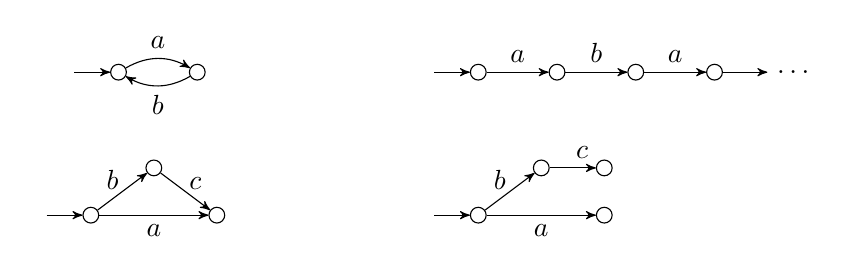
\begin{tikzpicture}[>=stealth']
    \begin{scope}
      \node[state, initial] (0) at (0,0) {};
      \node[state] (1) at (1,0) {};
      \path (0) edge[out=30, in=150] node[above] {$a$} (1);
      \path (1) edge[out=210, in=-30] node[below] {$b$} (0);
    \end{scope}
    \begin{scope}[xshift=13em]
      \node[state, initial] (0) at (0,0) {};
      \foreach \x in {1,2,3}
      \node[state] (\x) at (\x,0) {};
      \node (n) at (4,0) {$\dots$};
      \foreach \x/\y in {0/1,2/3}
      \path (\x) edge node[above] {$a$} (\y);
      \foreach \x/\y in {1/2}
      \path (\x) edge node[above] {$b$} (\y);
      \path (3) edge (n);
    \end{scope}
    \begin{scope}[yshift=-12ex, xshift=-1em]
      \node[state, initial] (0) at (0,0) {};
      \node[state] (1) at (.8,.6) {};
      \node[state] (2) at (1.6,0) {};
      \path (0) edge node[above, pos=.3] {$b$} (1);
      \path (1) edge node[above, pos=.7] {$c$} (2);
      \path (0) edge node[below] {$a$} (2);
    \end{scope}
    \begin{scope}[xshift=13em, yshift=-12ex]]
      \node[state, initial] (0) at (0,0) {};
      \node[state] (1) at (.8,.6) {};
      \node[state] (2a) at (1.6,.6) {};
      \node[state] (2b) at (1.6,0) {};
      \path (0) edge node[above, pos=.3] {$b$} (1);
      \path (1) edge node[above, pos=.7] {$c$} (2a);
      \path (0) edge node[below] {$a$} (2b);
    \end{scope}
  \end{tikzpicture}
\end{document}